\documentclass[border=0mm]{standalone}

\usepackage{tikz, xcolor}

%\renewcommand{\familydefault}{\sfdefault}

\definecolor{vq_grey}{RGB}{225,225,219}
%\definecolor{vq_grey_light}{RGB}{235,235,229}
%\definecolor{vq_grey_dark}{RGB}{215,215,209}

\pagecolor{white}



\begin{document}

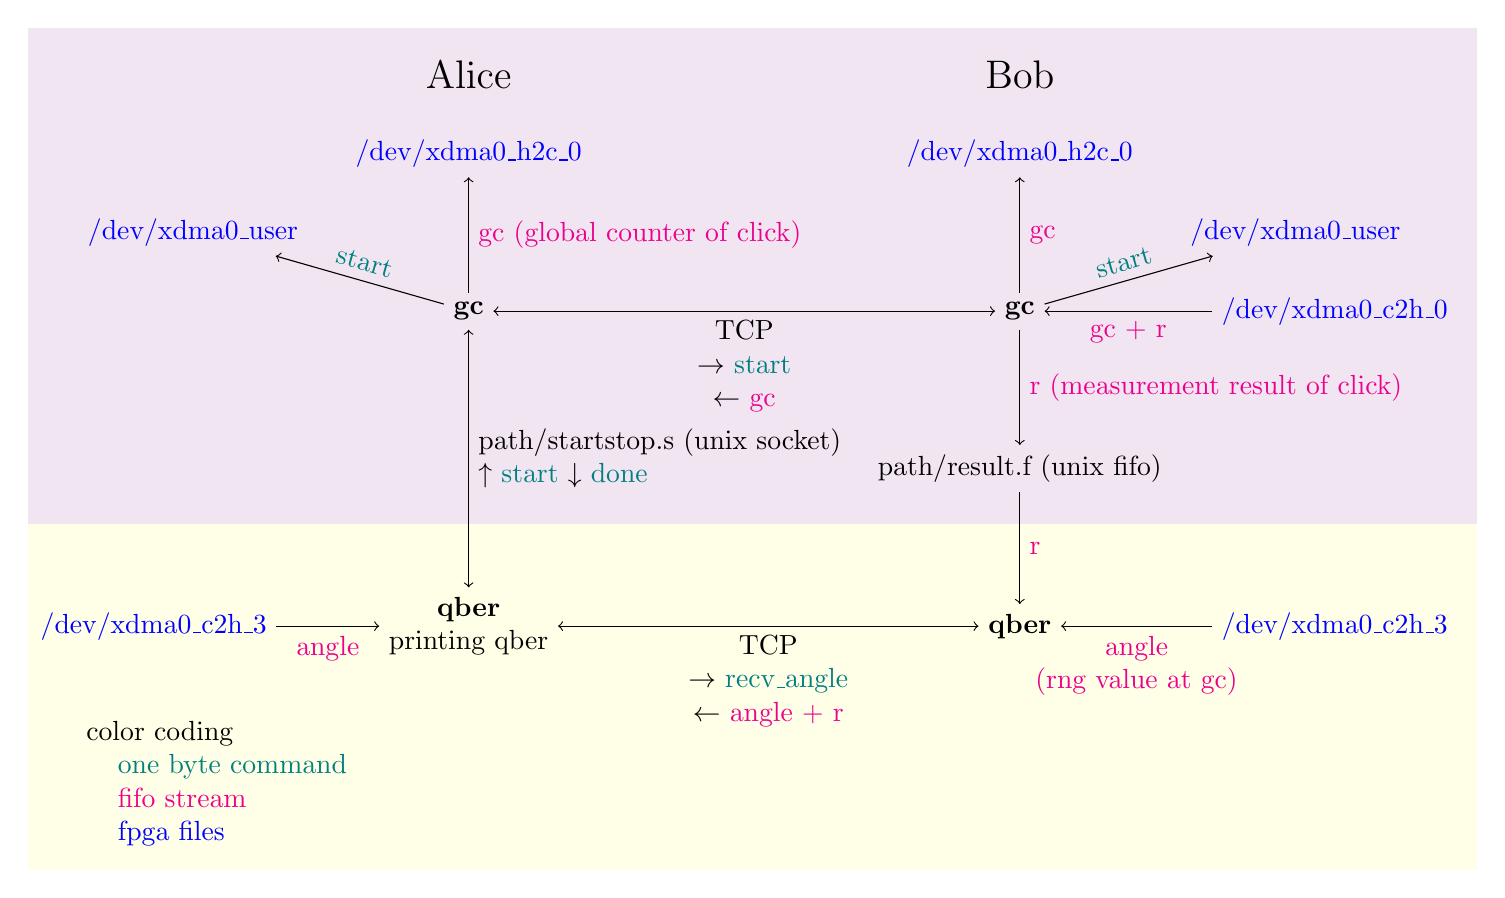
\begin{tikzpicture}

    \fill[violet!10] (-5.6,2.6) rectangle (12.8,-3.7);
    \fill[yellow!10] (-5.6,-3.7) rectangle (12.8,-8.1);


    \node at (0,2) {\Large Alice};
    \node at (7,2) {\Large Bob};

    \node[color=blue] (gcr) at (11, -1) {/dev/xdma0\_c2h\_0};
    \node[color=blue] (gcsb) at (7, 1) {/dev/xdma0\_h2c\_0};
    
    \node[color=blue] (gcsa) at (0, 1) {/dev/xdma0\_h2c\_0};
    \node[color=blue] (xdmaa) at (-3.5, 0) {/dev/xdma0\_user};
    \node[color=blue] (xdmab) at (10.5, 0) {/dev/xdma0\_user};

    \node(gcc) at (0,-1) {\textbf{gc}};
    \node(gcs) at (7,-1) {\textbf{gc}};

    \draw[<->] (gcc) -- (gcs) node(tcp)[below, midway, align=center]{TCP\\$\rightarrow$ \textcolor{teal}{start} \\$\leftarrow$ \textcolor{magenta}{gc}};

    
    \node(qberc) at (0,-5) [align=center] {\textbf{qber}\\printing qber};
    \node(qbers) at (7,-5) {\textbf{qber}};
    
    \node[color=blue] (aa) at (-4,-5) {/dev/xdma0\_c2h\_3};
    \draw[->] (aa) -- (qberc) node[midway, below]{\textcolor{magenta}{angle}};
    
    \node[color=blue] (ab) at (11,-5) {/dev/xdma0\_c2h\_3};
    \draw[->] (ab) -- (qbers) node[midway, below, align=center]{\textcolor{magenta}{angle}\\\textcolor{magenta}{(rng value at gc)}};
    
\draw[<->] (qberc) -- (qbers) node[below, midway, align=center]{TCP\\$\rightarrow$ \textcolor{teal}{recv\_angle}\\$\leftarrow$ \textcolor{magenta}{angle + r}};
    
    \draw[<->] (qberc) -- (gcc) node[midway, right, align=left]{path/startstop.s (unix socket) \\ $\uparrow$ \textcolor{teal}{start} $\downarrow$ \textcolor{teal}{done}};

    \node (rf) at (7,-3) {path/result.f (unix fifo)};
    
    \draw[->] (gcs) -- (rf) node[midway, right]{\textcolor{magenta}{r (measurement result of click)}};
    \draw[->] (rf) -- (qbers) node[midway, right]{\textcolor{magenta}{r}};

    \draw[->] (gcr) -- (gcs) node[midway, below, align=left]{\textcolor{magenta}{gc + r}};
    \draw[->] (gcs) -- (gcsb) node[midway, right]{\textcolor{magenta}{gc}};
    \draw[->] (gcc) -- (gcsa) node[midway, right]{\textcolor{magenta}{gc (global counter of click)}};
    
    \draw[->] (gcc) -- (xdmaa) node[midway, above, sloped]{\textcolor{teal}{start}};
    \draw[->] (gcs) -- (xdmab) node[midway, above, sloped]{\textcolor{teal}{start}};

    \node at (-3, -7) [align=left]{\hspace{-0.4cm}color coding\\\textcolor{teal}{one byte command}\\\textcolor{magenta}{fifo stream}\\\textcolor{blue}{fpga files}};





\end{tikzpicture}


\end{document}







